\documentclass[12pt]{article}

\usepackage{amsmath,amsthm,amsfonts,amssymb,amsxtra}
\usepackage{pgf,tikz}
\usepackage{multicol}
\usetikzlibrary{arrows}
\renewcommand{\theenumi}{(\alph{enumi})} 
\renewcommand{\labelenumi}{\theenumi}

\pagestyle{empty}
\setlength{\textwidth}{7in}
\setlength{\oddsidemargin}{-0.5in}
\setlength{\topmargin}{-1.0in}
\setlength{\textheight}{9.5in}

\theoremstyle{definition}
\newtheorem{problem}{Problem}

\makeatletter
\newcommand*{\radiobutton}{%
  \@ifstar{\@radiobutton0}{\@radiobutton1}%
}
\newcommand*{\@radiobutton}[1]{%
  \begin{tikzpicture}
    \pgfmathsetlengthmacro\radius{height("X")/2}
    \draw[radius=\radius] circle;
    \ifcase#1 \fill[radius=.6*\radius] circle;\fi
  \end{tikzpicture}%
}
\makeatother

\begin{document}

\noindent{\large\bf MATH 122}\hfill{\large\bf Final Exam}\hfill{\large\bf
  Fall 2017}\hfill{\large\bf Page 1/8}\hrule

\bigskip
\begin{center}
  \begin{tabular}{|ll|}
    \hline & \cr
    {\bf Name: } & \makebox[12cm]{\hrulefill}\cr & \cr
    {\bf VIP ID:} & \makebox[12cm]{\hrulefill}\cr & \cr
    \hline
  \end{tabular}
\end{center}
\begin{itemize}
\item Write your name and VIP ID in the space provided above.
\item The test has eight (8) pages, including this one, not counting the formula sheet attached at the end.  
\item You may remove the formula sheet as soon as the proctor instructs so.
\item Credit for each problem is given in parentheses at the right of the problem number. 
\item You must show sufficient work to justify all answers except on multiple-choice questions.  Correct answers with inconsistent or no work will not be given credit.
\item No books or notes may be used on this test.
\item No scratch paper is allowed.  You may use the last page of this booklet for that purpose.
\item An approved calculator may be used on this test.
\end{itemize}
\hrule

\begin{center}
  \begin{tabular}{|c|c|c|}
    \hline
    &&\cr
    {\large\bf Page} & {\large\bf Max.~points} & {\large\bf Your points} \cr
    &&\cr
    \hline
    &&\cr
    {\Large 2} & \Large 16 & \cr
    &&\cr
    \hline
    &&\cr
    {\Large 3} & \Large 12 & \cr
    &&\cr
    \hline
    &&\cr
    {\Large 4} & \Large 28 & \cr
    &&\cr
    \hline
    &&\cr
    {\Large 5} & \Large 20 & \cr
    &&\cr
    \hline
    &&\cr
    {\Large 6} & \Large 12 & \cr
    &&\cr
    \hline
    &&\cr
    {\Large 7} & \Large 12 & \cr
    &&\cr
    \hline\hline
    &&\cr
    {\large\bf Total} & \Large 100 & \cr
    &&\cr
    \hline
  \end{tabular}
\end{center}

\newpage

%%%%%%%%%%%%%%%%%%%%%%%%%%%%%%%%%%%%% Page 2
\noindent{\large\bf MATH 122}\hfill{\large\bf Final Exam}\hfill{\large\bf
  Fall 2017}\hfill{\large\bf Page 2/8}\hrule

\bigskip

\begin{problem}[4 pts]
The cost and revenue functions for a company are given by $C=1000+3.75q$ and $R=6.25q$ respectively.
The fixed costs of the company are:
\begin{multicols}{2}
\begin{center}
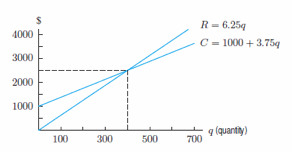
\includegraphics[width=\linewidth]{1graph1.png}
\end{center}
\begin{itemize}
\item[\radiobutton] \$1,000
\item[\radiobutton] \$3.75
\item[\radiobutton] \$400
\item[\radiobutton] \$6.25
\item[\radiobutton] \$0
\item[\radiobutton] \$2,500
\end{itemize}
\end{multicols}
\end{problem}

\hrule
\begin{problem}[4 pts]
When a person goes into shock, the cardiac output, in liters of blood per minute, decreases. One person’s cardiac output is 12 liters per minute when the person first goes into shock, and decreases by 2 liters per minute every hour that the person is in shock. Write a formula for cardiac output $C$ as a function of $t$, the time in hours since a person first went into shock.
\begin{itemize}
\item[\radiobutton] $C = 12 - 2t$
\item[\radiobutton] $t = 12 - 2C$
\item[\radiobutton] $C = -2 + 12t$
\item[\radiobutton] $t = -2 + 12t$
\item[\radiobutton] $C = 12 + 2t$
\item[\radiobutton] $t = 12 + 2C$
\end{itemize}
\end{problem}
\hrule

\begin{problem}[4 pts each]
Evaluate the following integrals.
\begin{enumerate}
\item $\displaystyle{\int_{0}^{4} \ln(y^2 + 5) \, dy} = $
\item $\displaystyle{\int_{10}^{103} 7xe^{30x^2}\, dx = }$
\vspace{7cm}
\end{enumerate}
\end{problem}

\newpage

%%%%%%%%%%%%%%%%%%%%%%%%%%%%%%%%%%%%% Page 3
\noindent{\large\bf MATH 122}\hfill{\large\bf Final Exam}\hfill{\large\bf
  Fall 2017}\hfill{\large\bf Page 3/8}\hrule

\bigskip

\begin{problem}[4 pts]
If the graph below is that of $f'(x)$, which of the following statements is true concerning the function $f(x)$?
\begin{multicols}{2}
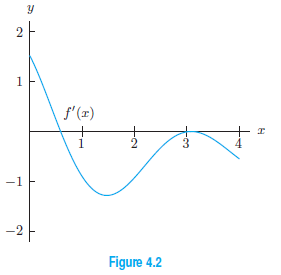
\includegraphics{3graph2}
\vspace{2cm}

\begin{itemize}
\item[\radiobutton] The derivative is zero at two values of $x$, both being local maxima.
\item[\radiobutton] The derivative is zero at two values of $x$, one is a local maximum, while the other is a local minimum.
\item[\radiobutton] The derivative is zero at two values of $x$, one is a local minimum on the interval, while the other is neither a local maximum nor a minimum.
\item[\radiobutton] The derivative is zero only at one value of $x$, where it is a local minimum.
\item[\radiobutton] None of the above.
\end{itemize}
\end{multicols}
\end{problem}

\hrule
\begin{problem}[4 pts]
Find all local max, min, and inflection points of $f(x) = 2x^3 + 3x^2-180x+9$.
\end{problem}
\vspace{6cm}
\hrule
\begin{problem}[4 pts]
Find the global maximum and the global minimum of $f(x) = 2x^3 - 9x^2$ over the interval $-1 \leq x \leq 6$.
\end{problem}

\newpage

%%%%%%%%%%%%%%%%%%%%%%%%%%%%%%%%%%%%% Page 4
\noindent{\large\bf MATH 122}\hfill{\large\bf Final Exam}\hfill{\large\bf
  Fall 2017}\hfill{\large\bf Page 4/8}\hrule

\bigskip

\bigskip
\begin{problem}[4 pts each]
Find the derivative of the following functions:
\begin{enumerate}
\item $f(x) = \sqrt{\dfrac{1}{x^{37}}}$
\begin{flushright}
  \begin{tikzpicture}
    \draw (-4cm,0.5cm) node {$f'(x)=$};
    \draw (-3cm,-0.2cm) rectangle (5cm,1.2cm);
  \end{tikzpicture}
\end{flushright}
\item $y = 5t^5 - 12\sqrt{t} + \frac{7}{t}$
\begin{flushright}
  \begin{tikzpicture}
    \draw (-4cm,0.5cm) node {$y'(t)=$};
    \draw (-3cm,-0.2cm) rectangle (5cm,1.2cm);
  \end{tikzpicture}
\end{flushright}
\item $f(x) = (3^x + x^4)(3 - \ln x)$
\begin{flushright}
  \begin{tikzpicture}
    \draw (-4cm,0.5cm) node {$f'(x)=$};
    \draw (-3cm,-0.2cm) rectangle (5cm,1.2cm);
  \end{tikzpicture}
\end{flushright}
\item $f(x) = \dfrac{x^6+4}{x}$
\begin{flushright}
  \begin{tikzpicture}
    \draw (-4cm,0.5cm) node {$f'(x)=$};
    \draw (-3cm,-0.2cm) rectangle (5cm,1.2cm);
  \end{tikzpicture}
\end{flushright}
\item $f(x) = \ln \big(18 - e^{-x}\big)$
\begin{flushright}
  \begin{tikzpicture}
    \draw (-4cm,0.5cm) node {$f'(x)=$};
    \draw (-3cm,-0.2cm) rectangle (5cm,1.2cm);
  \end{tikzpicture}
\end{flushright}
\item $f(x) = \big( 7 + \ln x \big)^{0.7}$
\begin{flushright}
  \begin{tikzpicture}
    \draw (-4cm,0.5cm) node {$f'(x)=$};
    \draw (-3cm,-0.2cm) rectangle (5cm,1.2cm);
  \end{tikzpicture}
\end{flushright}
\item $f(x) = 7e^{2x} + e^{-x^4}$
\begin{flushright}
  \begin{tikzpicture}
    \draw (-4cm,0.5cm) node {$f'(x)=$};
    \draw (-3cm,-0.2cm) rectangle (5cm,1.2cm);
  \end{tikzpicture}
\end{flushright}
\end{enumerate}
\end{problem}

\newpage

%%%%%%%%%%%%%%%%%%%%%%%%%%%%%%%%%%%%% Page 5
\noindent{\large\bf MATH 122}\hfill{\large\bf Final Exam}\hfill{\large\bf
  Fall 2017}\hfill{\large\bf Page 5/8}\hrule

\bigskip 

\begin{problem}[4 pts each]
Compute the antiderivative of the following functions:
\item $\displaystyle{\int x^4 (5 - 3x^5)^{12}\, dx =}$
\vspace{2cm}
\item $\displaystyle{\int  10xe^{x^2} \, dx =}$
\vspace{2cm}
\item $\displaystyle{\int \frac{7x^2}{(6x^3-2)^5} dx =}$
\vspace{4cm}
\item $\displaystyle{\int \frac{dx}{4-x} =}$
\vspace{4cm}
\item $\displaystyle{\int x^2 3^{5x^2}\, dx =}$
\end{problem}

\newpage

%%%%%%%%%%%%%%%%%%%%%%%%%%%%%%%%%%%%% Page 6
\noindent{\large\bf MATH 122}\hfill{\large\bf Final Exam}\hfill{\large\bf
  Fall 2017}\hfill{\large\bf Page 6/8}\hrule

\bigskip 

\begin{problem}[4 pts]
The following table shows sales of the medicinal herb saw palmetto, in millions of dollars, for several different years.  
\begin{center}
\begin{tabular}{|l||c|c|c|c|c|}
\hline
Year & 1997 & 1998 & 1999 & 2000 & 2001 \\ \hline
Sales & 85  &  107 &  116 &  122 &  123 \\ \hline
\end{tabular}
\end{center}
The \textbf{average rate of change} of sales over the period 1997 to 2001 is:
\begin{itemize}
\item[\radiobutton] 123 million dollars/year
\item[\radiobutton] 123 million dollars
\item[\radiobutton] 38 million dollars/year
\item[\radiobutton] 38 million dollars
\item[\radiobutton] 9.5 million dollars/year
\item[\radiobutton] 9.5 million dollars
\end{itemize}
\end{problem}

\hrule

\begin{problem}[4 pts]
What is the \textbf{average value} of $f(x) = \displaystyle{\sqrt{\vphantom{\lvert} 9-x^2}}$ over the interval $0 \leq x \leq 3$? 
\end{problem}
\vspace{4cm}
\hrule

\begin{problem}[4 pts]
For a product, the demand curve is $p=53-q^2$ and the supply curve is $p=3+q^2$, where $q$ is quantity and $p$ is price in dollars per unit. Find the \textbf{consumer surplus} when the market is in equilibrium (round your anwer to the nearest dollar).
\end{problem}

\newpage

%%%%%%%%%%%%%%%%%%%%%%%%%%%%%%%%%%%%% Page 7
\noindent{\large\bf MATH 122}\hfill{\large\bf Final Exam}\hfill{\large\bf
  Fall 2017}\hfill{\large\bf Page 7/8}\hrule

\bigskip

\begin{problem}[4 pts]
If $t$ is years since 1990, one model of the population of the worlds, $P$, in billions, is
\begin{equation*} P = \frac{40}{1+11e^{-0.08t}} \end{equation*}
\begin{enumerate}
  \item What does this model predict for the maximum sustainable population of the world?
  \vspace{1cm}
  \item According to this model, when will the earth's population reach 30 billion?
\end{enumerate}

\vspace{1cm}
\end{problem}
\hrule

\begin{problem}[4 pts]
At a price of \$80 for a half-day trip, a white-water rafting company attracts 300 customers.  Every \$2 decrease in price attracts an additional 12 customers.  What price should the company charge per trip to maximize revenue?
\vspace{7cm}
\hrule

\begin{problem}[4 pts]
The marginal cost function of producing $q$ mountain bikes is 
\begin{equation*}
MC(q) = \frac{600}{0.3q+5}.
\end{equation*}
If the fixed cost in producing the bicycles is \$2000, find the total cost to produce 30 bicycles.
\end{problem}

\end{problem}

\newpage

%%%%%%%%%%%%%%%%%%%%%%%%%%%%%%%%%%%%% Page 8
\noindent{\large\bf MATH 122}\hfill{\large\bf Final Exam}\hfill{\large\bf
  Fall 2017}\hfill{\large\bf Page 8/8}\hrule

\end{document}

%%% Local Variables:
%%% mode: latex
%%% TeX-master: t
%%% End:
